\documentclass[openany,twoside]{memoir}

\usepackage{fontspec}
\usepackage[no-sscript,no-logos]{xltxtra}
\usepackage{fancyhdr,tabu,refstyle,varioref,pgfplots,pgfplotstable,graphicx,titlesec,enumitem}
\usepackage[autostyle]{csquotes}
\usepackage[strict,notes,backend=biber]{biblatex-chicago}
\usepackage[multiple,marginal,bottom]{footmisc}

\setlrmargins{*}{4cm}{*}

\addbibresource{citations.bib}
\setromanfont[Mapping=tex-text]{Linux Libertine O}
\setlength{\headheight}{15.2pt}
\setlength{\belowcaptionskip}{10pt}
\counterwithout{figure}{chapter}

\setcounter{secnumdepth}{-1}
\setcounter{tocdepth}{2}

\setitemize{itemsep=0pt,topsep=0pt}

\titlespacing*{\chapter}{0pt}{*0}{*0}

\titleformat{\chapter}[hang]{\normalfont\huge\bfseries}{}{0pt}{}

\DefineBibliographyStrings{english}{%
   bibliography = {References},
}

\pagestyle{fancy}
\fancyhf{}
\renewcommand{\headrulewidth}{0pt}

\begin{document}
\begin{Spacing}{2}
\title{On the Nature of Political Interaction as Conversation}
\author{Sam Stuewe\\[50ex] Edited and Reviewed by\\ Professor David Blaney\\ Professor Andrew Latham\\ Professor Terry Boychuk}
\date{}
\pagenumbering{gobble}
\maketitle
\chapter{Contents}
\makeatletter
\@starttoc{toc}
\makeatother
\makeatletter
\addtocontents{toc}{\vspace{-20pt}}
\chapter{List of Figures}
\@starttoc{lof}
\makeatother
\newpage

\pagenumbering{arabic}

\fancyhead[L]{Political Interaction as Conversation}
\fancyhead[R]{\nouppercase{\leftmark}}
\fancyfoot[C]{–\,\thepage\,–}

\addtocontents{toc}{\vspace{-20pt}}
\chapter{Abstract}
\thispagestyle{fancy}
Unlike many previous theories (which privilege prediction), this thesis aims to facilitate understanding complex political interactions through a simple and accessible metaphor of conversation (drawing on various precursory theories from geopolitics to constructivism). 
To explore the facility of this framework, I analyze the Occupy protests' lasting effects in localities, the United States overall and internationally. 
Through my analysis, whether or not Occupy was “successful,” it is clear that it has had a lasting effect on modern political interaction. 
Despite its limitations, the metaphor's versatility and extensibility may allow it to remain useful for analyzing many diverse cases.

\addtocontents{toc}{\vspace{-20pt}}
\chapter{Acknowledgments}
\thispagestyle{fancy}
This project is the culmination of a great deal of work by many people; I would be remiss if I did not adequately thank them.
First, allow me to begin by thanking my advisor and chair of my defense panel, David Blaney.
Over the course of this last year, Professor Blaney has been instrumental in helping me to shape and polish this project.
In addition, both Professors Andrew Latham and Terry Boychuk, David's fellow examiners, have offered much assistance in the initial and final steps of producing a workable document.
Finally, but certainly not of small contribution, both Lucas Allen in particular, a fellow honors student, and the whole honors colloquium helped significantly in the early stages of writing and served as a great source of catharsis and support throughout the year.

This project, however, was not just the result of academic commitment.
Both my family and close friends have helped support me through the whole process and I cannot thank them enough for their help.
Furthermore, I completed this paper using a wide variety of software, \oldstylenums{100} percent of which consisted of free and open-source projects.
The following open-source projects were used in the creation of this document:

\end{Spacing}\begin{itemize}
   \item{\XeLaTeX\,and \emph{biblatex} for document processing and citation management}
   \item{VIm (``Vi Improved''), a text editor}
   \item{Linux Libertine and Inconsolata, free and open-source fonts}
   \item{git, a version control system used for tracking edits}
   \item{zathura, a \textsc{pdf} viewer}
\end{itemize}
\begin{Spacing}{2}

\addtocontents{toc}{\vspace{-20pt}}
\chapter{Introduction}
\thispagestyle{fancy}
Political thinkers often create metaphors to characterize political interaction parsimoniously.
The Realist tradition may have created the most basic metaphor for this purpose: the Billiards table.
Each actor is cast as a solid Billiards ball whose inner-workings are of no concern to analysts.
The interactions between the balls are reduced to rolling around and running into one another (which may be helpful or hindering).\footcite{mearsheimer01}
Like many of the metaphors that would follow, this framework intentionally dismisses a great deal of complexity\footnote{
For example, this metaphor never speaks to what force is holding the cue which forces the balls to move.}
in favor of simplicity.
The argument for such a framework is that the simplicity allows analysts to make solid predictions by simplifying complex situations.
However, as the saying goes, ``The Devil is in the details.''
Dismissing complexity in exchange for simplicity only creates models with limited application.
More ``leftist'' political theories, such as social constructivism, refrain from over-simplifications and allow a great deal more complexity.
Unfortunately, they often lead to such high-level abstraction that it becomes difficult for lay persons (or even modern politicians) to apply them.

Perhaps unsurprisingly,\footnote{
It could be argued that political interaction has become significantly more complex with globalization and the rise of the Internet age.}
modern political interactions have become more and more difficult to categorize which has made their analysis much more complex.
The ``Arab Spring,'' and the Occupy movements (widely, and problematically, categorized as ``protest politics'') best exemplify the complex situations with which political frameworks struggle.
Realism largely disregards these movements as unimportant.\footnote{
States are the primary (often, the only) important actors.
Thus, any process or movement which takes place at a lower level is not worth analysis.}
Social constructivism, on the other hand, often discusses the structures which give rise to the protests and the systems in which they operate.
Unfortunately, the focus on the system's influence robs the protests of their agency.
It even ignores the fundamental principles of the protests (advocating for an escape and reformation of the structures themselves, not their subordinate policies).

It seems clear that, to tackle the analysis of such complex movements, a new framework is needed which provides an elegant way to understand interactions without dismissing their complexity.
In this paper, I will propose one such new framework in an attempt to bridge the gap between the simply understandable and the overly complex.
The metaphor I will propose---of political interaction as conversation---has been in use for a long while but appears to have not yet been formalized as a framework.
To achieve its goal, to provide a level of depth and complexity such that a wide variety of interactions may be fruitfully analyzed while remaining accessible enough for non-theorists to find it useful, it must expressly not focus on prediction.
In stark contrast to many previous political frameworks, particularly \emph{realpolitik}, my framework will \emph{only} facilitate understanding and analysis.
That is, creating a generalized framework that focuses on making predictions will either over-simplify their cases till the predictions no longer seem applicable for real-world interactions, or will become so complicated in its construction that any elegance is lost.
The framework I propose, therefore, will avoid predictive applications altogether.\footnote{
If this framework, by coincidence, should manage to become useful for predicting outcomes of various interactions, that would be an unexpected benefit, but it is not an explicit goal of this thesis.}

Through this framework, I will argue that the Occupy protests represented a radical new manifestation and application of conversation.
Further, I will argue that Occupy is a scalable phenomenon and, therefore, may be applicable to international contexts. 
Before attending to the primary pieces of this argument, I will first construct the framework based on interactions cast as conversations by drawing on and extending previous theories.
Both the framework and an accompanying model I will propose shortly after will speak indirectly to many of the strategies and organizational structures involved in Occupy (e.g., the decision-making processes, public outreach and media campaigns, etc.).
Before addressing the primary pieces of this argument, I will first construct and propose the new framework mentioned above and an accompanying model.
Using the framework and model for political interactions, I will move on to address the primary argument regarding Occupy.
In addressing Occupy as a case-study, I will view it as three separate contexts: local, nation-wide and international.
For the local case, I will accept OccupyWallStreet as the best option.\footnote{
OccupyWallStreet has been studied the most extensively (and was so during the primary occupations as well).
Furthermore, it had the most media attention and participants.
Even if it were not remotely the best example of a local Occupy movement, it is the easiest to study, and therefore, the easiest to use for drawing conclusions.}
Next, I will look at Occupy as a relatively cohesive movement nationally in the United States (in terms of overarching similarities and in terms of effects specific to Occupy in its national context).
Finally, I will attempt to view Occupy as a movement on a global scale.
Each context, operating on a different scale, has different characteristics (and, unfortunately, widely different sets of available data).
Though each case's analysis is confined by available data, they all include examples of statements which fit my model and, subsequently, support the underpinning framework.

\chapter{Theoretical Background}
\thispagestyle{fancy}
\section{Intellectual Origins}
\seclabel{origins}
This framework draws its origins from a wide variety of theoretical traditions---from geopolitics to various constructivist traditions.
It synthesizes three fundamental pieces of analysis which are each used by various previous theories.
They can be succinctly summarized as ``where a conversation takes place,'' ``who participates in the conversation,'' and ``what is said and how.''
These three fundamental pieces, I would argue, form the set of characteristics applicable to any given conversation (a metaphor which will be elaborated in the next main section).
The following three subsections will explore the origins of each fundamental piece and some of the shortcomings of each initial application.

\subsection{Location}
The notion of an arena in which political interactions take place is not new and the exact meaning of the term has not always been well-defined. 
For some political scientists, it defines, at its most basic level, a sense of scope---e.g., the ``international arena.'' 
However, for Henry Mintzberg, an arena is less a definition of scope as much as it is a description of duration. 
In his text ``The Organization as Political Arena,"\footcite{mintzberg85} Mintzberg refers to arenas as being particular situations of political interaction characterized by a form of organized conflict. 
He posits a typology of political arenas for which the defining characteristics differentiating the cases are the organization of the arena and how it is constituted (primarily in terms of the intensity of the conflict, how well contained the conflict remains and for how long the conflict lasts).\footcite[141]{mintzberg85} 
Mintzberg's typology is founded upon the notion that all organizations are oriented around conflict and that because of the trends of conflict in politics.\footcite{mintzberg85}

The most useful component of this model is its simplicity. 
As with other seemingly predictive models, given various input factors (of which there are not many possibilities)\footnote{
Mintzberg's typology only allows for four different organizations with very little variance}, 
probable outcomes may be predicted with confidence. 
But the notion of a political arena as being only valuable with reference to conflict implicitly dismisses cooperative political interaction;\footcite[152]{mintzberg85} and, even more distressing, his model assumes a vacuum-sealed environment. 
That is, there is little to no context shaping the arena before the conflict becomes apparent. 
No political interaction is without context and without giving some analysis focused on the context which gave rise to, or influenced, the interactions themselves, a great deal of useful information (which will assuredly affect outcomes) is lost.
A more helpful theory of location would establish the relationship between the different types of arenas as culminations of various contextual factors which guide the evolution of the arena itself and which influence the eventual participants and actions which take place in it.

Giving an extra dimension to the contextuality of interactions, Anthony Giddens's theory of ``structuration''\footcite{giddens86} offers a model for understanding the existence of institutionalization.
In particular, Giddens traces the unintended consequences of a given action as it becomes a condition which influences future actions.
However, because of their having arisen unintentionally, they are overlooked or unacknowledged in the calculus of future actions.\footcite[5]{giddens86}
The repetition of this cycle leads to the embedding of these unacknowledged action-influencing conditions, or institutionalization.
This notion of institutionalization brought about through overlooked conditions is at the heart of the concept of normalization---an integral part of understanding how institutions become internalized.
Though Giddens speaks at great length about the separations between intended and unintended consequences, he glosses over the possibility for \emph{intended} consequences to play into the same framework of overlooked conditions which internalize norms.
That is, it is entirely conceivable that a political actor could influence future actions through intentional decisions which would still go overlooked by other actors. 

More important than these notions of internalization, however, is Giddens's argument surrounding the ``duality of structure.''\footcite[16]{giddens86}
Through this mechanism, Giddens argues that not only do institutions shape future actions, but each action reproduces the institution (which may be reinforcing or modifying).\footcite[19]{giddens86}
Thus, the institutions which constrain action are created and recreated by action itself.
Such a simple concept can revolutionize structural theories.
In the past, constructivism cast actors as characters acting within structures with little, if any, form of escape.
Furthermore, these structures were often considered static or unchanging.\footnote{
Obviously inaccurate given the vastly changing nature of structural contexts over time.}
Giddens's revision gifts agency back to actors; that is, structures significantly guide actions, but they are not static---in fact, actors are capable and \emph{do} directly affect structures in this process of recreation.
Through Giddens, now we have a basic feedback loop through which structures can change over time and through the actions of participants.

Drawing on Mintzberg and Giddens, the notion of a political arena---of a location in which political discussion\footnote{
For the sake of this thesis, a ``discussion'' will be defined as a political interaction focusing on a single topic.
As a result, ``conversations'' can be said to be made up of one or more ``discussions,'' just as discussions are made up of one or more statements.}
can take place---has three basic characteristics.
First, it is organized and created by actors who shape its character.
Second, the organization and structure of the location influence (sometimes obviously, and other times subversively) future actions taken.
Finally, the organization and the action are mutually generative and reinforcing---each produces and reproduces the other.
With this basic concept of where conversations take place in mind, it is necessary to step forward to see what theorists say about the participants in interaction.

\subsection{Participants}
While the location and context of any political interaction holds great importance, those who participate in the interaction itself are, perhaps, the primary subjects of interest. 
Toward the beginning of \emph{A Semisovereign People}, E. E. Schattschneider, like Mintzberg, frames political interaction as conflict and confrontation as it relates to participants.\footcite{schattschneider75} 
In particular, his model focuses on an argument taking place in a hotel lobby.\footcite[1--5. Ironically, despite mentioning the location of the conflict, Schattschneider fails to discuss how the location may have affected the interaction.]{schattschneider75} 
In this argument, as in Schattschneider's framework as a whole, the focus should be placed on the ``audience,'' not the ``speakers.'' 
He pays special attention to the size of the audience as this is what, he claims, will play the decisive role in determining the outcome of the conflict: 
\end{Spacing}
\blockquote{The logical consequence of the foregoing analysis of conflict is that the balance of forces in any conflict is not a fixed equation until \emph{everyone} is involved. 
If one tenth of \oldstylenums{1} percent of the public is involved in conflict, the latent force of the audience is \oldstylenums{999} times as great as the active force, and the outcome of the conflict depends overwhelmingly on what the \oldstylenums{99.9} percent do. 
Characteristically, the potentially involved are more numerous than those actually involved. 
This analysis has a bearing on the relations between the ``interested'' and the ``uninterested'' segments of the community and sheds light on interest theories of politics. 
It is hazardous to assume that the spectators are uninterested because a free society maximizes the contagion of conflict; it invites intervention and gives a high priority to the participation of the public in conflict.\footcite[5]{schattschneider75}}\begin{Spacing}{2}
\noindent
Here, Schattschneider offers a great number of helpful ideas. 
For example, he offers us the concept of interest as it relates to the audience as valid participants.
Perhaps most important, he makes obvious that the dynamics of an interaction are ever-changing. 

Unfortunately, Schattschneider's model focuses almost entirely on the participants (and, even then, very heavily on the audience and not the vocal participants). 
Furthermore, not all political interaction can be accurately characterized as conflict. 
With this conflation of interaction as conflict and the disregard for any unit of analysis aside from participants, Schattschneider's model fails to capture a large number of cases and ignores a number of factors present in any given conversation.

Combining some of Schattschneider's insights with the basic concept of a location, the concept of participant dynamics begins to take shape.
Though Schattschneider places a (perhaps undue) large emphasis on the non-vocal participants, it is clear that the relationships between participants in the conversation matters a great deal, and that the construction of the location might have serious implications as to the status of those relationships.

Susan Bickford, similar to Schattschneider and Mintzberg, still assumes a level of conflict evident in political interaction but focuses on a different aspect of participants and their relation to the conversation as a whole.
In particular, her text \emph{The Dissonance of Democracy}\footcite{bickford96} focuses on listening and how much it affects conversations disproportionate to how much it has been addressed in academic literature. 
Referencing Plato's \emph{Republic}, Bickford argues that communicative interaction is founded on the understanding that those making arguments will have an audience willing to listen.\footcite[3]{bickford96}
This realization is extremely useful as it offers a basic cast of participants and their roles in a conversation.
Fundamentally speaking, arguments rely on having multiple participants who play various roles (moving between speaker and listener).
Beyond this realization, it highlights an extremely powerful action for audience members to take: not listening.\footcite[3]{bickford96}
Bickford notes that pre-cursory agreements determine rules of interaction such that various means of decision-making become normalized.\footcite[3--5. Simply put, these pre-cursory agreements can be understood as ``constitutions''---both formal and informal institutions which govern interaction.]{bickford96}
These agreements are often made to prefer some ``peaceful'' form of decision making rather than relying on the use of force.

Bickford's argument is particularly useful because it does not empower ``listening'' to the disenfranchisement of ``speech,'' but rather equalizes the playing field, claiming that politics itself is ``about the dynamic between the two.''\footcite[4]{bickford96}
Furthermore, she does not assume conflict is the only character of interaction.
She asserts a complex understanding of relationships (both connections and divisions) which influence actions through affecting the dynamics of any given conversation.\footcite[9--11]{bickford96}

Now, with the addition of Bickford's notion of speech and listening as being complimentary and the roles associated with both activities, the dynamics between participants are far more clear.
Coupled with the notion of presence as it relates to position in a given location (particularly that a given position may tip the scales of influence in favor of the participant which holds that position), the stage is set for the possibility of discussions taking place between these participants to be weighted in favor of particular parties, and for those discussions to be heavily shaped by the context in which they arise.
Thus, I turn to the content of the conversations itself and how discussions of content have evolved in academic literature.

\subsection{Content}
With his focus set on this final aspect of political interaction, Jeffrey Banks's \emph{Signaling Games in Political Science} concentrates on information transmission, or ``signaling.''\footcite{banks91} 
Banks's analysis focuses on signaling games (particularly incomplete information signal games\footnote{
He argues that models which allow for complete information have very little predictive and intellectual merit due to serious limitations on the applicability of the model in real situations})
and how political interaction can be cast in the light of these games. 
Despite his focus on game theory (which emphasizes predictiveness), Banks still offers a prototypical model of politics as conversation. 
In his case analysis, he cast the model's ``players'' as speakers and the signals sent which may influence other players' actions as ``speeches.''\footcite[37]{banks91} 
For Banks, there are two well-defined players, the ``sender'' and ``receiver,'' and there is little acknowledgment of any response.\footcite[4]{banks91} 
That is, where Banks imagines, at most, a one-directional message being sent, a more realistic metaphor would describe messages being sent back and forth between multiple participants which often mutually influence one another. 

Banks's model also greatly limits the scope of its application through its implicit definitions. 
For example, the only signals Banks concerns himself with are those which influence others by limiting the receiver's set of choices through a mechanism he refers to as ``agenda control.''\footcite[3]{banks91} 
Not only does this cut out all cases of interaction in which the effects are undetermined, but it undermines the understanding of interactions as being more than just unidirectional. 

Furthermore, Banks's notion of influence houses a very traditional definition of power.
His notion of ``agenda control'' could be imagined as an application of Lukes's second dimension or as Barnett and Duvall's first type.\footcite{lukes05, barnettduvall05}
That is, the only form of power that actors have in Banks's model is very reminiscent of traditional realism (when actor A makes actor B do something they would otherwise not do).
Later in his explanation, he modernizes it somewhat to account for indirectly affecting signals sent and received (crossing into Barnett and Duvall's second type).
Yet, he still never accounts for more abstract forms of power (e.g., ``forming consent'' or ``creating people''), and surprisingly still never captures the ``mobilization of bias,'' though ``non-decisions.''\footcite{schattschneider75}
All these limitations are made for the sake of the model's simplicity (and therefore, the ease of its application for prediction) but are detrimental to its sophistication and thus negate much of its practical relevance.

Despite all the limitations Banks places on his model, it remains surprisingly versatile. 
In his case analysis, he applies his model to literal cases (candidates making speeches to audiences) but makes it generalizable through a metaphor by which analysts may understand much higher-level games through the same terms. 
This is what makes Banks's model so appealing despite its limitations: it is scalable.
That is to say, Banks clearly creates many (perhaps) artificial constraints on his model in the name of predictiveness, but the model itself is helpful for understanding situations which he would never have considered.
In particular, his notions and the language he uses surrounding the concept of signaling are useful for describing any action made at any scale of interaction (be it between individuals or between nation-states).

Adding Banks's insights into the content of a conversation to the more complex picture of participant dynamics that Bickford offers creates a much more helpful understanding of how conversation is conducted.
Conversation takes place when messages are sent between participants who then interpret them and respond.
Each message is influenced not just by the sender(s) and receiver(s), but also by the environment which has brought the participants together and established the dynamics and context for the conversation in the first place.
In the next section, I will offer a metaphor---founded in the terms which have been used throughout the paper up to this point---to help clarify the relationship between each aspect of conversation.

\section{Conversation as a Metaphor}
In their seminal work on metaphor, George Lakoff and Mark Johnson argue that metaphors are deeply pervasive and that humans fundamentally rely upon metaphor.\footcite[3--6]{lakoffjohnson80}
Throughout their text, \emph{Metaphors We Live By}, they seek to show the use of metaphor as being applicable to a great many aspects of human life.
With their framework of metaphor in mind, I will attempt to construct a unified framework for political interaction grounded primarily in a ``structural'' metaphor of conversation.\footcite[14]{lakoffjohnson80} 
The inherent advantage of this type framework is that it draws on a construct that would be simple for any academic or lay reader to access, analyze, \emph{and} extend.
Thus, I will attempt to create a selectively comprehensive (and inherently extensible) framework for political interaction using this metaphor. 
However, despite its not covering all cases or explaining all phenomena, any intellectual extension of the framework should be discoverable through little more than logical exploration.

This metaphor of conversation has three general components which were discussed throughout section 2.
These are the \emph{location}, the \emph{participants} and the \emph{content}.
Without discussing all three components, vital information---which may be critical to useful analysis or generalization---is lost.
Each author discussed before has offered a number of valuable concepts which, when developed further and are synthesized, offer a far more realistic and revealing picture of political interaction.
What follows is the initial construct of a metaphor of conversation for political interaction drawing on this synthesis.

\subsection{Imagine a Room}
In this room, there are an indeterminate number of walls, doors and windows.
Some of the walls have been added in such a way that they form small enclaves within the larger room itself.
Both the doors and windows vary between open and closed states; and on occasion, some are removed entirely or are newly installed.
The room itself was built a long time ago (though there was never an exact moment when construction was started).\footnote{
Though it is outside the scope of this work to establish, the concept of a well-defined line between a ``state of nature'' and modern society has been soundly questioned. 
To reflect this, assume that this room has been evolving through construction and maintenance without a clearly defined beginning.}
Due to the construction and previous alterations, this room's acoustics and floor are uneven which amplify some voices while effectively muting others. 
Finally, despite this room's having changed (significantly) over time, alterations made to the room take a great deal of time to complete, and often happen as individual projects to change very small characteristics.

This room is far from empty. 
There are many people inside at any given moment whose focus varies greatly.
Some of these people are focused on discussions taking place within the room itself, while others are more concerned with those going on outside.
There are also, of course, some people outside the room looking in through a window or open door, and many people will either move from the inside out or vice versa quite often.
Regardless of where people are in the room, they serve two roles (often simultaneously): that of the speaker and that of the listener.\footcite[4]{bickford96}
Like any other room, movement inside is fairly unencumbered (which allows for some ability to mobilize groups of support during debates). 
Each person is given an assigned seat, which rarely changes, where they are expected to sit for most discussions.\footnote{
Though they are \emph{expected} to sit in their assigned position for the most part, they are not (typically) physically required to do so.}
Seating assignments are shaped by the placement of furniture throughout the room, and one's position in the room affect one's capacity to be heard and ability to hear others.\footnote{
It may even be the case that the better able one is to hear others, the less able they are to be heard.}

Understanding that the characteristics of the room and the people inside it have a great deal of influence on the topic, imagine a discussion taking place in this room.
Its organization is governed by the physical limitations of the room and by agreements made between participants.\footnote{
Which are created through discussions held before-hand (e.g., the seating arrangement)}
Though the topic is often determined by those inside the room taking part in the discussion, it may concern those outside as well.
The topic of discussion may morph and change as various statements are made.
Various people in the room will understand the topic in a different light, which will color their speaking about and listening to discussion concerning it.
Statements and questions made will often be of a certain tone which reflects the speakers' opinions surrounding the topic.
And, the tone of various statements can greatly affect the responses which they may garner.
Each discussion in this room may seem as though it has a well-defined beginning and end, but such is not the case.
Discussions often (if not, always) flow from one into another even if they do not fundamentally change either the room or its participants.

\subsection{Grounding the Metaphor}
The locational aspect of this metaphorical room serves to represent the systems of rules, norms and physical limitations which govern modern political interaction.
These norms and systems were ``created''\footnote{
A problematic term because it validates the view that a well-defined moment of consensus which brought humankind out of a state of nature and into society---a fiction.} 
long ago and have been evolving ever since.
Some of these systems are pervasive enough to have become internalized (or, at least, self-reinforcing)\footcite[Like mobilizing bias in][]{schattschneider75} where others remain only because participants agree to them.\footcite[Reminiscent of pre-cursory agreements discussed by][]{bickford96}
The walls, windows and doors highlight the separations---which are often artificial in nature---between those involved in the conversation and those who are not.
Furthermore, the notion of enclaves establishes the possibility of separations between participants who are \emph{all} involved in the conversation.\footnote{
These could be embodied by ideological groupings like political parties, or by demographic subpopulations like ethnicity.}
The openness of the doors and windows are meant to make clear the traversability of these artificial boundaries and allow for a basic mechanism for joining and leaving a given discussion.
But the interior of the walls describe a separate characteristic.
The acoustics of a room (i.e., how sound reverberates through a space) are heavily determined by the arrangement, construction and decoration of the walls.\footcite{giddens86}
With little modification to the walls alone, a room can be made to amplify or mute sound coming from a particular point.
These acoustics serve to demonstrate how an institution (physical or abstract) might benefit the voice of some over others solely because of their relative position.
In deeper detail still, the varying height of the floor provides, perhaps, a more obvious example of the lack of equality in constructs of conversation.
The final metaphorical detail I offer about the room itself establishes a sense of longevity.\footcite{mintzberg85,giddens86}
While the metaphor explicitly allows for participation to change drastically, and discussion contents are nothing but ephemeral, the construction itself (though it can be modified) resists drastic change.

In contrast to the locational aspect, the participational aspect of the metaphor represents the focus, relationships and possible actions which describe the participants in a given discussion.
The focus of the participants speaks to their attentiveness to particular conversations or traits of those conversations---for example, are participants actively engaged in a conversation, or are they more interested in one taking place further away (or even one taking place outside the room itself)?\footcite{bickford96}
Despite how attentive a participant may be, however, they will still be part of a conversation by means of either their active or passive presence.\footcite{bickford96,giddens86}
Entering and exiting the room is an extension of the dichotomy of presence and absence; namely, it offers a simple mechanism by which participants can remove their influence (whatever influence they may have) from the conversation,\footnote{
Perhaps ironically, or maybe just fascinatingly, this willful departure from asserting direct influence is itself a statement made in the conversation which may carry great power.} 
or by which they may attempt to assert influence by entering the room having been outside.
The motion within the room and the seating arrangement are meant to evoke an understanding that participants inside the room have \emph{some} autonomy.
As various conversations may be taking place at any given moment in the room (or in its enclaves), participants may wander so that they may hear better.
Of course, this freedom of movement is largely cosmetic; to change one's position in the room permanently is much more difficult as it is a matter of structural change.\footcite{giddens86}

Finally, the content-oriented aspect represents the organization, topic, tone and duration of the conversation itself.
All pieces of this aspect are determined almost entirely by location and participation.
However, influence on content from location and participation is not limited to those inside the room; those outside may have a great deal of influence on the topic as well.\footcite[Perhaps, on occasion, more so than those inside? cf.][]{bickford96, giddens86}
Unlike the relative stability of the room itself and even more obvious than the fluidity of change in the participants, the nature of the conversation can change very swiftly.
Each singular statement made by a participant may be enough to shift the topic, and, to complicate the matter, the different identities of the participants will influence how they interpret the topic (and how their contributions are interpreted by others).\footcite{banks91, bickford96}
As intertwined as the rest, the tone of the conversation as a whole derives from the tone with which each participant makes a statement.
Thus, should participants speak with a tone of hostility, the conversation may take on that character as a whole.
Finally, the notion that discussions are not well-defined and never truly end reinforces the understanding that the process of a conversation does not end: each statement leads to further development which leads to more statements.\footcite{schattschneider75, bickford96}

\section{Statements in Conversation}
Given this more complex (but still general) understanding of how conversations are created and how they unfold, I would like to turn the analysis of conversation in the direction of what type of statements can be, and are, made during a discussion.
Before I discuss the categorization and subsequent typology associated with statements, it is important to note that the term ``statement'' may be metaphorical or literal.
Each statement might be something \emph{literally said} by a person in the sense that Bickford and Mintzberg discuss, or could be as abstract as the speeches which concern Banks.\footcite{bickford96,mintzberg85,banks91}
However, the language and rationale for understanding that a conversation derives from discussions made up of statements, in either the metaphorical or literal sense, remains the same.

Thus, I turn towards a typology of statements.
Each statement in a discussion may be categorized with reference to affecting the scope of one of the three aspects of a conversation mentioned earlier.
A statement can either widen, make any cosmetic change or narrow the location, the participation and the content of a given discussion.\footnote{
These are only the most basic forms which statements can take.
There is room for statements to fit into multiple categories (e.g., alternatives or renovations which remove some element and add something in its place).
Furthermore, as the time it takes to complete a statement may vary, it is entirely possible for a statement to interrupt one made previous.
These are only a few of the possible extensions to this typology---I have little doubt that more could be added.}
The following table illustrates fairly broad categories that attempts to capture how widening, cosmetic change and narrowing may take place.
The horizontal axis describes which aspect is being affected by the statement whereas the vertical axis describes how that aspect is being affected.
For example, ``construction'' refers to the category of statements which \emph{widen} the \emph{location}; and, conversely, ``specification'' refers to the category of statements which \emph{narrow} the \emph{content}.
In the sections which follow the table, I will elaborate on how each type of statement can take shape and the effects it can have on the dynamics of a conversation.

\addtocontents{lof}{\vspace{10pt}} % may need to be -10pt
\begin{figure}
   \tabulinesep=1.5mm
   \centering
   \caption{Statements categorized by what they modify and how}
      \begin{tabu} [c] {c|c|c|c|} \everyrow{\tabucline{2-4}}
         \multicolumn{1}{c}{} & \multicolumn{1}{c}{Location} & \multicolumn{1}{c}{Participants} & \multicolumn{1}{c}{Content} \\
         Widening & Construction & Inclusion & Generalization \\
         Cosmetic & Maintenance & Rearranging & Rephrasing \\
         Narrowing & Demolition & Exclusion & Specification \\
      \end{tabu}
   \label{typology}
\end{figure}

\subsection{Location}
As mentioned briefly in the metaphor elaborated in the section above, modifications made to a location take a fair amount of time and energy compared to those relating to the other aspects.
Typically, these statements are made because participants believe each addition allows for more equity.\footnote{
That is, not what is truly equal, but rather, what they consider to be \emph{fair}.}
These modifications can take the shape of construction, maintenance and demolition.
Construction, logically, involves the addition of a new installation to the room.
New additions can be anything from a new wall, window, doorway or even a small enclave or adjoining room.
Because of the amount of work required (along with the implications of the new separations, or entrances), these tend to be some of the most difficult statements to support.
Perhaps one of the best examples of construction in the sphere of international relations can be found by looking to the United Nations Security Council.\footcite{un45}
The \textsc{unsc} is given the power to establish subsidiary bodies as needed under the \textsc{un} Charter.\footcite{un45}
Over the years, a great many new subsidiaries have been created, primarily in the form of committees.
Each of these committees can be viewed as enclaves inside the room of the \textsc{unsc}; each may have several (seemingly) independent discussions taking place within at any given moment, but all of them are influenced and shaped by the larger context which gave rise to them.
In turn, each committee influences policy and rhetoric present in the \textsc{unsc} overall.

Unlike construction, maintenance focuses not on making drastic changes through creating new additions, but rather on reforming or revising those installations which have already been created.
Maintenance often takes the form of modifying the various heights of the floor or changing the acoustics of the room's walls through soundboards.
It is not uncommon for these statements of maintenance to reverse or reinforce previous pieces of maintenance.
These statements also have a strong chance of influencing indoor dynamics, but their effects do not appreciably increase or decrease the size of the room itself.
Again, one of the most obvious manifestations of maintenance lies in the history of the \textsc{un}---the formation of the United nations Human Rights Council.
The \textsc{unhrc} was established to replace a heavily criticized organization, the United Nations Human Rights Commission.
The goals of both were largely the same, but the structure of varied greatly.\footcite{bbc06}
This represented not a drastic addition of a new installation, but rather focused on reforming an older one.\footnote{
This is, perhaps, a better example of renovation or alternative than simply maintenance, but the primary difference between renovation and maintenance is solely a degree of magnitude.}

Finally, demolition is the process of removing established installations.
Anything that can be added in construction can be removed in demolition (including the foundational structures of the room itself).
Though these statements can be controversial because they remove installations which have become part of the established order, they often involve much simpler proposals since they focus only on removal of an installation which may take much less work than the planning for an addition.\footnote{
Aside from the example of the \textsc{chr} mentioned above, the only other example I was able to locate within the \textsc{un} was the removal of the International Refugee Organization (\textsc{iro}) in favor of the United Nations High Commissioner for Refugees (\textsc{unhcr}).
The \textsc{iro} appears to be an identical case to the \textsc{chr}.}

\subsection{Participants}
Much like statements which affect the makeup of the location of a conversation, those that affect the makeup of the participants can be categorized by their affect on its extent.
It is important to note that these statements are made much more often and are completed much more quickly than those which affect the location overall because the room, in general, facilitates movement.
These statements will either take the shape of inclusion, rearrangements or exclusion.
Statements of inclusion most typically come to bear in the form of invitations from, or demands made by, the indoor participants to entities currently outside or vice versa.
However, they may involve invitations or acceptance of participants into smaller enclaves as well.\footnote{
The relationship between each enclave and the larger room is similar to the relationship between a conversation and a discussion.
Each room is likely to have one or more enclaves which, in most ways, share all the same characteristics that the room itself has (e.g., walls, doors, windows, etc.).
Also like the room, particular statements and characteristics are welcome within each enclave while others are excluded.}
For example, one could look to the inclusion of nations as member states to the United Nations.
Every new nation recognized as a member state is invited inside, so to speak.
With the inclusion of a new member, many organizations may be refactored to adjust to the new member, or the new member will adjust to the organizations in-place already.
However, the primary change is in the makeup and dynamic of the membership; each new member brings a new perspective and a new set of interests to the conversation.

Rearrangements, the more cosmetic change, most often affect the seating arrangement or speaking order of a given conversation.
These can drastically affect position in the room and can therefore make fundamental changes to the dynamics between participants in a given conversation.
However, because they do not affect who is welcome in a conversation and who is excluded, they will be far less controversial than inclusionary or exclusionary statements.\footnote{
Must come up with a good example of this---\textsc{unsc} rotating membership?}
A good example of this may be found the rotating membership of the \textsc{unsc}.
Though the \textsc{unsc} is, in many ways, an enclave within the \textsc{un} and, therefore, being invited to join the \textsc{unsc} is a form of inclusion,\footnote{
Or, perhaps, their more minor role means they represent \emph{demands} for greater inclusion rather than inclusion itself.}   
the rotating members serve a largely cosmetic role.\footnote{
I do not mean to offend.
The utility and function of the \textsc{unsc}'s rotating membership are not the focus of this paper, nor this section.}
As a result, the rotating membership tend to be positions that do not significantly change the relationship between nations and, thus, represent little more than cosmetic changes.\footnote{
Note that some changes that seem similar, on the surface, may be significantly different.
For example, additions or removals from the permanent membership of the \textsc{unsc} would have far more significant effects.}

Finally, exclusionary statements are those which intentionally remove a participant from membership in the room itself or in a smaller enclave.
These statements may be made in order to exclude an individual, or they may be made by an individual to exclude themselves.\footnote{Hirschman and Fraser with exiting}
By again looking to the \textsc{unsc}, there is a simple example to be found.
Recently,\footcite{worth13} Saudi Arabia was invited to take one of the rotating seats of the \textsc{unsc}, and declined.
In doing so, Saudi Arabia chose to exclude itself from the position offered.
This action may have been entirely rhetorical---i.e., an attempt to signal a lack of need for the \textsc{unsc}---but Saudi Arabia's Foreign Ministry released a statement noting that it declined because the \textsc{unsc} has proven to be ineffective and that it would gladly join the conversation were the body to prove itself useful.\footcite{worth13}

\subsection{Content}
Even more than participational statements, content-oriented statements are much more quickly made than those which concern the location.
Each single discussion can involve a great deal of these statements, and each statement has wide ranging immediate effects on the future of a discussion's content.
These statements most often take the forms of generalization, rephrasing and specification.
Generalizations are made to widen the content of the conversation by allowing for a greater variety of allowed statements.
That is, often through manipulation of terms or the topic itself, generalizations offer an avenue for more areas of discussion to be a part of the conversation.
Arguably, the best modern example of topic expansion arose with the Occupy movement.
In order to help bring about public discussion of issues that concerned many people of very different backgrounds, the issues important to each person were framed as being important to everyone.
That is, the topic of discussion was open-ended; anyone who wished to air a grievance was welcome to do so.\footcite{graeber11}

However, many times a statement is not well-received not because its scope is too wide or too narrow, but rather just because of how it was phrased.
As a result, cosmetic change arises in the form of simple rephrasing.
Rephrasing a statement can be as simple as using different terminology, but the motions of doing so may make the statement itself much more acceptable by other participants.\footnote{
A similar example may be found in the case of ``wealth inequality'' and ``income inequality;'' two phrases which I will explore in more depth in my case studies.}

Finally, content-oriented statements may be made to narrow the topic through specifications.
Specifications, like generalizations, may be made through the terms of the conversation or more powerfully through the topic itself.
Making these statements can cause future statements to be more efficient by focusing them on more specific goals; however, doing so will necessitate that other goals be left unattended.

Over the course of the next section, I will seek to analyze the Occupy movement on varying levels of effect in terms of the typology explicated above.
In particular, I will focus on several watershed moments of the movement, their lasting effects, and some examples of messages which never got the recognition that the more pervasive messages did.
Occupy must be recognized as a movement with an effect on, at least, three different levels of interaction: metropolitan, national and international.
In this section, I will offer a short history of Occupy itself and then delve into the intricacies of each level as a separate case.
Each case applied different strategies---and, as a result, different statements---which colored the effectiveness of each message and, when viewed in terms of the framework and typology laid out above, make clear the lasting effects.

\chapter{Case Studies}
\thispagestyle{fancy}
\section{A brief history of Occupy}
In light of the Arab Spring protests and various occupations in Greece and Spain, Adbusters (an online blog with a history of social justice motivations) began calling for similar movements to happen in the United States.\footcite{adbusters11}
That is, Adbusters advocated for protests highlighting inequalities and other issues of civil interest that government bodies appear to have ignored.
On \oldstylenums{17 September 2011}, the occupation of Zuccotti Park began, and the Occupy movement in the United States was born under the banner of a Twitter hashtag (\#OccupyWallStreet).
Over the course of the next several months, similar occupations began in cities across the United States such as Washington, \textsc{d.c.}, Kansas City, \textsc{mo}, and Saint Paul, \textsc{mn}.\footcite[For a list of Occupy locations, see ][]{wikipedia14} 

Through the use of consensus-based General Assemblies, the various occupations each had their own focus on issues they felt central to improving life for all people in the United States.
Each General Assembly also served as a semi-centralized forum for making decisions on behalf of the collective occupation.
The areas of decision-making ranged from stances on various issues to over-arching ideological stances.
And, for each issue area, a committee was created---using very similar mechanics---which would meet ahead of time to determine the most important topics to be proposed at the Assemblies.
For an example of the issue areas, one of the primary misconceptions held about Occupy was that it was a movement without express purpose.\footcite{rice11}
This perception most likely arises from Occupy's lack of advocacy for a particular policy.
Contrary to popular belief, this lack of clear policy advocacy was entirely intentional.
One of the earliest committees formed was one concerning policy advocacy.
However, the Assembly overall remained resolute that the real problems the movement should address could not be resolved through normal policy channels (and require systemic change).

Not long after the occupations began, several cities opted to evict the protesters from their locations (most notably the Wall Street eviction on 15 November).
Though slowed by the semi-forced transition away from physical occupation, the protest movement did not cease with the evictions.
Rather, the movement has shifted course significantly.
Now, rather than focusing on outright protests, Occupy has transformed significantly to lobby for social change through other means.

The next several sections will tackle three cases of Occupy (OccupyWallStreet, Occupy nationally in the United States, and Occupy internationally).
Unfortunately, the data available is not comparable for each case, so direct comparisons cannot be reliably made.
However, the goal of studying these cases is not comparative, but rather just exploring the validity of using the model and framework I proposed in the last chapter.
As a result, exploring the available data for each case (comparable to the other cases or not) should be enough to offer some insight to the relevance of the theory to reality.

\section{Wall Street}
Occupy in the United States is most well-known for Occupy Wall Street (\textsc{ows}).
This is not only because it was the first in the series, but also because of how the movement spread through the public eye.
Information spread about Occupy often using one hashtag, \#OccupyWallStreet, even though it did not correctly highlight the separation between each site.
Even news media focused most heavily on the protests in Zuccotti Park.
This being the first, and largest of the protests, it is arguably the best location to use as an example of a local-level case.

\subsection{Initial Occupation}
The initial occupation of Wall Street serves as one of the most easily catagorizable statements made throughout the whole Occupy movement.
Upon the achievement of consensus that the current structure of society and government fails to address issues of civil interest, the decision is made to help construct a new space for discussion that might fill the void.
This piece of construction was focused at addressing, among other things, the inequality perceived in the realm of discourse.
Thus, the movement never sought to elect candidates to office---it was never a goal of Occupy to change politics from inside the current system.
Rather, \textsc{ows} created a space \emph{outside} normal politics meant to facilitate systemic change \emph{inside}.

Yet, Occupy is not solely a manifestation of construction.
After the occupation itself began, the rhetorical strategies employed were crafted to embody the messages of the change they hope to create.
That is, \textsc{ows} sought to practice what it preached by realizing some of the social changes it hoped to see nationally in its own governance.
Most obvious, from an analytic standpoint, would be the direct nature\footnote{
It is misleading to say that Occupy supported direct democratic involvement. 
Democracy is founded on the notion of majority-rule; Occupy was founded on the notion of consensus. 
Democracy is not ``democratic'' enough.} 
of the decision-making structure of the occupation itself, but that is likely not the most well-known example.
Perhaps the best-known example of this ``practice what you preach'' policy was the ``\oldstylenums{99} percent'' slogan.
Occupy saw a great many people (the overwhelming majority, in fact) as having almost no voice in their government and with no capacity to change such a reality.
The use of the ``\oldstylenums{99 percent}'' slogan was meant to energize and mobilize the very population it refers to (i.e., everyone save those who allegedly already control politics\footnote{
This is not meant to be so politically charged, but rather highlight that Occupy used this slogan to convey a sense of empowerment to the public.}).

Beyond construction, the occupation's system of self-governance through General Assemblies served as a statement of inclusion---one meant to help incorporate the disenchanted and disenfranchised members of society into the discussion so that they might have increased agency.
By doing so, \textsc{ows} reaffirmed its concentration on mass political involvement, but even more, it began the groundwork to create new (and strengthen established) communities which continue to work for the betterment of society.

\subsection{Responses to Occupy}
In short order, ``wealth inequality'' had been identified as one of the primary causes for many of the problems identified.
However, Occupy remained intent on being a forum for the spread of information and awareness, not an actor advocating for specific policy change.
Perhaps due to frustration with the movement's lack of a clear policy goal, or maybe simply because of the inconvenience, Michael Bloomberg, Mayor of New York City, decided that the occupation must end.
Regardless of the motivations, the eviction was clearly a statement in itself.

At first glance, the eviction appeared as a statement of demolition---as seeking to remove the space that had been created for the new discourse.
Yet, it cannot be so simply classified.
One of the cited motivations for the evictions was a need to clean Zuccotti Park of hazardous materials and to keep the premises safe.
It is worth noting that Zuccotti Park is private property. 
This status has serious implications for the legality of the occupation, but oddly, it never became a decisive issue.
It does, however, lend serious legitimacy to the eviction.
One of the reasons the eviction did not take place sooner was because Zuccotti Park was private property---the government had no authority to remove any person from the premises unless illegal activity was suspected or at the request of the owner. 
This means that the eviction must have, at the very least, been approved by the owner---it may have even been requested.
After the cleaning was completed, the protesters were allowed to return to the park, though new regulations had been added stipulating that protesters may not lie down or sleep in the Park.
Given that the space was reopened for protesters to use, it may be best to characterize the evictions not as statements of demolition, but rather as statements of maintenance---made to keep the new space up to standard by constraining the movement through regulation.

On the other hand, the new restrictions implemented effectively destroyed any option for an extended physical occupation.
In that sense, the evictions were not maintenance so much as they were demolition mixed with exclusion.
By implementing restrictions that severely decreased the time that people can spend in protest, the number of people able to participate was also significantly lessened.\footcite{barronmoynihan11}
Though a large majority of Occupiers were found to be relatively wealthy individuals,\footcite[10]{milkman13} a considerable number of them were homeless.
With no ability to physically occupy the Park for extended time, many could not stay in the area at all.\footnote{
\textsc{Ows} was not the only site to have such issues; OccupyMN (later OccupyMpls, or \textsc{ompls}) faced many of the same issues.}

\subsection{Working Forward}
Most fascinatingly, though Occupy did not end with the evictions (and there \emph{are} still physical occupations and protests that continue to the time of this writing), news organizations almost entirely ceased covering the movement.\footnote{
Perhaps this was because it became more difficult to track when it became less centralized (but this seems unlikely as the internal media organization and resources are just as easy to reach today as they were in the midst of the occupations)}
Each site had different means of working forward for social change after the evictions.
\textsc{Ows} emerged again almost a year later working with a more specific goal and a new name: OccupySandy.
They organized a relief effort in the wake of the hurricane that coordinated over \oldstylenums{50,000 volunteers and \$600,000} in donations.\footcite[35--36]{milkman13}
Of course, not all sites had natural disasters to respond to, but there is no shortage of social issues in the United States which were addressed.\footnote{
For example, in Minnesota, \textsc{ompls} eventually evolved into OccupyHomes, a movement to help leverage collective bargaining against unfair foreclosures.}

Localized in each city, Occupy focused on issues specific to the community.
However, on a larger scale, Occupy's mission was less concrete (perhaps leading to the eventual loss of steam the movement felt).
Yet, it seems the story on the national level is so vastly different than the localized accounts because the media's portrayal (and, subsequently, the public's reception) was colored so dependently by their relationship with different localized movements.
It was also heavily influenced by what appeared to be Occupy's lack of a coherent message.\footnote{
What I would argue was a miscommunication, but very important nonetheless.}

\section{The United States}
Nationally speaking, Occupy held an incredibly high amount of support from the general public.\footcite{cooper11}
Such high national support quickly curtailed after the movement became characterized as one populated by wealthy college students complaining about student loan debt.\footcite{bella12,zakarin11}
Regardless, several incidents across the localities had massive effects on the political climate of the Nation, overall.
This section will focus on several symbols that became common-place references across the nation through Occupy along with some of the national effects of the Occupy movement as a whole.

\subsection{Government Resistance}
\addtocontents{lof}{\vspace{-20pt}}
\begin{figure}[h]
   \centering
   \caption{Lt. John Pike pepper-sprays students}
   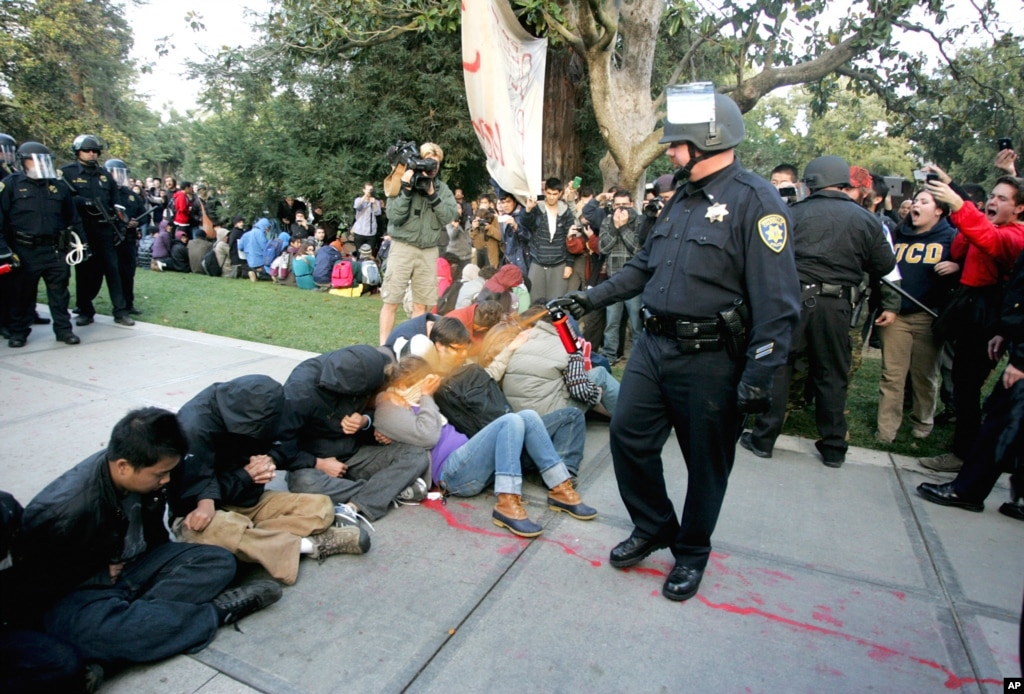
\includegraphics[width=4.25in]{graphics/pike.jpg}
   \label{spraycop}
\end{figure}

In \oldstylenums{figure~\ref{spraycop}}, one of the most widely recognizable pictures distributed during the primary occupations and the evictions, Lt. John Pike, of the University of California Davis police force, is using pepper spray on a number of peacefully assembled and protesting students.
This incident sparked outrage across the country, and, quickly, use of this picture as a symbol of government's oppressive response to the protests spread.
It, along with some of the political commentary about it, became so widely-known that it rose to the level of an ``internet meme.''\footcite{scott11}

All negative government response in the following several months would be characterized by this photo, particularly police actions (unsurprisingly).
Yet, Lt. Pike's actions were not heavily punished, and the scandal has fallen out of the public consciousness.
In fact, recently, Lt. Pike was awarded around \oldstylenums{\$38,000} in a settlement due to psychological trauma resulting from the incident---more than each of the students was awarded in the legal battle immediately following the incident.\footcite{goyette13}
As a result of the failure of memory, Lt. Pike's interaction with Occupy had very little lasting affect.
Much simpler messages had more staying power.

\subsection{Tracking the ``\oldstylenums{99} Percent''}
Arguably one of the clearest pieces of evidence that Occupy had a lasting impact on the political climate in the United States is the prevalence of particular phrases and concepts that, before Occupy, had been rarely mentioned, or were almost non-existant.\footcite[
Not all analysts agree, of course. 
For a more critical analysis of the staying power of terms used surrounding the Occupy movement, see][]{knefel12}
Some phrases had fairly minimal change, where others noticed massive increases.
The following charts show the highest percent relative prevalence\footnote{
This is a relative measure of prevalence comparing the number of searches of any given sample to the maximum number of searches made in the examined period.} 
of interest across each quarter per year from \oldstylenums{2009--2013}.\footnote{
Initially, each graph began tracking around \oldstylenums{2005} as that is how far the tracking data reaches.
However, for each of these terms, the trends shown from \oldstylenums{2005--2008} are almost identical to those from \oldstylenums{2009--2010}.
Despite the relative nature of this measure, since each graph includes the peak, the other data points are not significantly changed.
Should anyone be interested in investigating this data more thoroughly, the sets are all freely available from http://google.com/trends.}
The first phrase I investigated was ``wealth inequality.''

\begin{figure}[h]
   \centering
   \caption{Relative Prevalence of ``wealth inequality'' across \oldstylenums{2009--2013}}
      \begin{tikzpicture}
         \begin{axis}[xlabel=Year, 
                      ylabel=Percent, 
                      xticklabel style={/pgf/number format/1000 sep=}]
            \addplot [no markers, blue] table{
               X       Y
               2009.00 0
               2009.08 6
               2009.17 12
               2009.25 7
               2009.33 8
               2009.42 8
               2009.50 8
               2009.58 9
               2009.67 9
               2009.75 9
               2009.83 6
               2009.92 7
               2010.00 9
               2010.08 10
               2010.17 11
               2010.25 9
               2010.33 8
               2010.42 8
               2010.50 6
               2010.58 6
               2010.67 9
               2010.75 11
               2010.83 8
               2010.92 11
               2011.00 8
               2011.08 14
               2011.17 13
               2011.25 17
               2011.33 9
               2011.42 7
               2011.50 8
               2011.58 13
               2011.67 13
               2011.75 28
               2011.83 31
               2011.92 14
               2012.00 12
               2012.08 12
               2012.17 11
               2012.25 15
               2012.33 11
               2012.42 7
               2012.50 7
               2012.58 9
               2012.67 11
               2012.75 15
               2012.83 16
               2012.92 10
               2013.00 8
               2013.08 16
               2013.17 100
               2013.25 36
               2013.33 23
               2013.42 15
               2013.50 15
               2013.58 13
               2013.67 21
               2013.75 40
               2013.83 37
               2013.92 40
            };
         \end{axis}
      \end{tikzpicture}
   \label{wealthineq}
\end{figure}

\oldstylenums{Figure~\ref{wealthineq}} shows a fairly consistent prevalence across \oldstylenums{2009 through the beginning of 2011 between 4 and 10 percent}.
Across the next several months it spiked in interest as unrest grew over the rising concerns of nationally and individually held debt.
As Occupy took its place in public view, interest more than doubled to \oldstylenums{22} percent.
Unsurprisingly, the evictions and subsequent decline of Occupy's presence in the public consciousness coincided with a decline in interest of ``wealth inequality.''
However, for the most part, levels of interest during \oldstylenums{2012} remained higher than previous years.
Then, in the first half of \oldstylenums{2013}, a video\footnote{
http://www.youtube.com/watch?v=QPKKQnijnsM}
summarizing the state of wealth inequality in the United States, drawing on Dan Ariely's and Michael Norton's \oldstylenums{2011} study,\footcite{arielynorton11} went viral.
Though the video in-question was originally uploaded in November \oldstylenums{2012}, it seems that there was a short delay between its publishing and its virality.\footnote{
This is fascinating, and may be well worth the time of those who study virality.
Unfortunately, the notion of delayed virality is outside the topic of this paper.}
Given that the study was published in late \oldstylenums{2011} and makes no reference to the Occupy movement throughout its text, it would be very difficult to claim that the study itself was influenced by Occupy.

However, as the video which apparently caused the \oldstylenums{2013} spike does reference concepts propagated by the Occupy movement (e.g., ``the \oldstylenums{1} percent''), it is much easier to claim that there was, at least, some influence from Occupy present in this mass spread of interest.
It may be tempting for some to argue whether or not the video was caused by the study or by the movement, but such a discussion is beyond the purpose of this paper.
Even if there were a causal relationship between either the study or the protests and the video, proving so would be quite difficult.
The most important revelation is that Occupy's effect is clear.
This term, that had been rarely mentioned before the protests, now pervades modern political discussion.
At the moment, it appears that this impact is primarily a widening of content, i.e., generalization.
``Income inequality'' and ``wealth inequality'' are expressions of similar concepts.
However, though ``wealth inequality'' is a generalization of ``income inequality,'' it remains less pervasive in modern political discussion than ``income inequality.''
So, this generalization allows for a wider set of discussions without significantly rephrasing other topics.

Striking as this pattern is, ``wealth inequality'' had, at least, been discussed before Occupy got off the ground.
A better example of the shift would be tracking a phrase that had almost no exposure before the occupations.
The most obvious example of one such phrase is the now common-place term for the public---``the \oldstylenums{99} percent,''---discussed earlier.

\begin{figure}[h]
   \centering
   \caption{Relative Prevalence of ``the \oldstylenums{99} percent'' across \oldstylenums{2009--2013}}
      \begin{tikzpicture}
         \begin{axis}[xlabel=Year, 
                      ylabel=Percent, 
                      xticklabel style={/pgf/number format/1000 sep=}]
            \addplot [no markers, blue] table{
               X       Y
               2009.00 0
               2009.08 0
               2009.17 0
               2009.25 0
               2009.33 0
               2009.42 0
               2009.50 0
               2009.58 0
               2009.67 0
               2009.75 0
               2009.83 0
               2009.92 0
               2010.00 0
               2010.08 1
               2010.17 1
               2010.25 2
               2010.33 2
               2010.42 1
               2010.50 1
               2010.58 1
               2010.67 1
               2010.75 2
               2010.83 2
               2010.92 1
               2011.00 2
               2011.08 2
               2011.17 2
               2011.25 2
               2011.33 2
               2011.42 2
               2011.50 2
               2011.58 2
               2011.67 5
               2011.75 100
               2011.83 44
               2011.92 16
               2012.00 10
               2012.08 11
               2012.17 8
               2012.25 9
               2012.33 7
               2012.42 5
               2012.50 4
               2012.58 4
               2012.67 7
               2012.75 5
               2012.83 5
               2012.92 4
               2013.00 2
               2013.08 4
               2013.17 4
               2013.25 5
               2013.33 3
               2013.42 3
               2013.50 3
               2013.58 3
               2013.67 4
               2013.75 4
               2013.83 4
               2013.92 4
            };
         \end{axis}
      \end{tikzpicture}
   \label{99perc}
\end{figure}

Across the beginning of \oldstylenums{2009}, the phrase ``the \oldstylenums{99} percent'' was of almost no interest whatsoever.\footnote{
Again, this also appears to be the case stretching back to the beginning of \oldstylenums{2004}}
From the end of \oldstylenums{2009} through the middle of \oldstylenums{2011}, the prevalence of interest only increased to around \oldstylenums{2} percent.
However, this likely has no relation to the concepts to which the phrase now refers.
It is only with the birth of Occupy that this phrase sees any prevalence.
Very noticeably, as Occupy takes the stage in late \oldstylenums{2011}, this phrase receives more interest than at any other time.
Following the evictions and the decline of Occupy, interest in this phrase has declined significantly, now remaining stable around \oldstylenums{5} percent.
It should not be very surprising that a term so closely related to the movement itself declined so heavily after the movement is thought to have ended.
However, that the phrase is now a part of political discussions (particularly those surrounding wealth inequality), makes clear that Occupy left some mark.
Furthermore, the phrases prevalence is still more than double what it was before Occupy's inception.

Lately, this phrase has been co-opted for various goals, but the initial purpose was to widen the participation in political conversation.
That is, Occupy used the phrase ``the \oldstylenums{99} percent'' to convey a sense that the movement focused on issues of concern to the huge majority of the population.\footnote{
There is an alternate interpretation.
Rather than hoping to increase the participation, perhaps this statement had been mobilized to increase the movement's legitimacy by claiming to speak on behalf of \oldstylenums{99} percent of the public.
However, Occupy's open character and consensus-based model seem to suggest that the primary goal was involvement.}
The more recent appropriations of this phrase have been less focused on political involvement.
In fact, some of them relate more to marketing than to politics.
There have been a few product reviews which paint the products as being desirable because they are affordable ``even for the \oldstylenums{99} percent.''\footcite{khaw12}
The most fascinating quality of such articles is the blissful ignorance of the co-opted phrase's original implication of anti-capitalism.
Despite the use of the phrase to refer to a group absent any of the implications made by the reference, it still falls within the bounds of a reference that draws influence from Occupy (if only because the phrase itself was popularized by the protests).

Of course, phrases propagated by Occupy itself cannot adequately exemplify its national affects.
For a more complete analysis, it is necessary to also view the prevalence of some phrases propagated outside the movement.
Unfortunately, these phrases are far more difficult to identify because they are often phrases that have been used to refer to other similar movements in the past and are being reapplied to the movement rather than the reverse (being created to speak about the movement and then being applied in other situations in the future).
However, there are some that are still identifiable.
Perhaps unsurprisingly, these phrases are often those used to speak negatively about Occupy---``entitled,'' for instance.

\begin{figure}[h]
   \centering
   \caption{Relative Prevalence of ``entitled'' across \oldstylenums{2009--2013}}
      \begin{tikzpicture}
         \begin{axis}[xlabel=Year,
                      ylabel=Percent,
                      xticklabel style={/pgf/number format/1000 sep=}]
            \addplot [no markers, blue] table{
               X       Y
               2009.00 42
               2009.08 44
               2009.17 39
               2009.25 45
               2009.33 39
               2009.42 41
               2009.50 37
               2009.58 43
               2009.67 45
               2009.75 51
               2009.83 45
               2009.92 43
               2010.00 47
               2010.08 48
               2010.17 56
               2010.25 53
               2010.33 49
               2010.42 47
               2010.50 47
               2010.58 45
               2010.67 52
               2010.75 48
               2010.83 50
               2010.92 45
               2011.00 54
               2011.08 55
               2011.17 55
               2011.25 52
               2011.33 55
               2011.42 57
               2011.50 54
               2011.58 48
               2011.67 100
               2011.75 69
               2011.83 62
               2011.92 49
               2012.00 60
               2012.08 62
               2012.17 54
               2012.25 66
               2012.33 63
               2012.42 56
               2012.50 61
               2012.58 64
               2012.67 71
               2012.75 69
               2012.83 64
               2012.92 58
               2013.00 61
               2013.08 64
               2013.17 62
               2013.25 68
               2013.33 62
               2013.42 57
               2013.50 58
               2013.58 56
               2013.67 66
               2013.75 72
               2013.83 66
               2013.92 61
            };
            \addplot [no markers, red] table[y={create col/linear regression={y=Y}}]{
               X       Y
               2009.00 42
               2009.08 44
               2009.17 39
               2009.25 45
               2009.33 39
               2009.42 41
               2009.50 37
               2009.58 43
               2009.67 45
               2009.75 51
               2009.83 45
               2009.92 43
               2010.00 47
               2010.08 48
               2010.17 56
               2010.25 53
               2010.33 49
               2010.42 47
               2010.50 47
               2010.58 45
               2010.67 52
               2010.75 48
               2010.83 50
               2010.92 45
               2011.00 54
               2011.08 55
               2011.17 55
               2011.25 52
               2011.33 55
               2011.42 57
               2011.50 54
               2011.58 48
               2011.67 100
               2011.75 69
               2011.83 62
               2011.92 49
               2012.00 60
               2012.08 62
               2012.17 54
               2012.25 66
               2012.33 63
               2012.42 56
               2012.50 61
               2012.58 64
               2012.67 71
               2012.75 69
               2012.83 64
               2012.92 58
               2013.00 61
               2013.08 64
               2013.17 62
               2013.25 68
               2013.33 62
               2013.42 57
               2013.50 58
               2013.58 56
               2013.67 66
               2013.75 72
               2013.83 66
               2013.92 61
            };
         \end{axis}
      \end{tikzpicture}
   \label{entitled}
\end{figure}

\oldstylenums{Figure~\ref{entitled}} clearly shows the presence of the term \emph{before} the Occupy movements took shape.\footnote{
Note that this graph's lowest value is \oldstylenums{40} percent, unlike the previous graphs which find their lowest value in single-digit numbers.}
However, the prevalence of ``entitled'' clearly saw an increase during the occupations.
In fact, during September \oldstylenums{2011}, the term saw its highest prevalence on-record.
This seems to suggest that there was some relationship between Occupy and the use of this term.
The difficulty in analyzing this graph arrives after Occupy's eviction.
The interest in the term following Occupy's decline has clearly increased, but is the increase actually related to Occupy, or was Occupy's affect on the term's interest an anomaly?

To make this analysis simpler, \oldstylenums{figure~\ref{entitled}} includes a linear regression.
The regression, surprisingly or not, seems to demonstrate the anomalous nature of the \oldstylenums{2011} spike.
If Occupy had a significant affect on the overall prevalence of this term, I would expect to see a much steeper slope of the regression line.
Despite the obvious spike in prevalence that appears related to Occupy, it seems that in the case of this term, Occupy does not appear to have significantly changed the interest in the term ``entitled.''
As least in reference to Occupy, use of this term appeared to be a statement of exclusion (narrowing of participation).
That is, opponents of Occupy wished to delegitimize (and, subsequently, remove) it.

\begin{figure}[h]
   \centering
   \caption{Relative Prevalence of ``anarchy'' across \oldstylenums{2009--2013}}
      \begin{tikzpicture}
         \begin{axis}[xlabel=Year,
                      ylabel=Percent,
                      xticklabel style={/pgf/number format/1000 sep=}]
            \addplot [no markers, blue] table{
               X       Y
               2009.00 11
               2009.08 11
               2009.17 10
               2009.25 10
               2009.33 9
               2009.42 9
               2009.50 9
               2009.58 18
               2009.67 43
               2009.75 34
               2009.83 39
               2009.92 30
               2010.00 15
               2010.08 13
               2010.17 13
               2010.25 12
               2010.33 12
               2010.42 12
               2010.50 13
               2010.58 17
               2010.67 43
               2010.75 34
               2010.83 28
               2010.92 25
               2011.00 16
               2011.08 14
               2011.17 13
               2011.25 24
               2011.33 24
               2011.42 22
               2011.50 23
               2011.58 29
               2011.67 61
               2011.75 45
               2011.83 55
               2011.92 42
               2012.00 28
               2012.08 22
               2012.17 20
               2012.25 17
               2012.33 20
               2012.42 21
               2012.50 25
               2012.58 31
               2012.67 100
               2012.75 69
               2012.83 61
               2012.92 47
               2013.00 31
               2013.08 24
               2013.17 23
               2013.25 20
               2013.33 20
               2013.42 21
               2013.50 27
               2013.58 34
               2013.67 91
               2013.75 65
               2013.83 64
               2013.92 67
            };
            \addplot [no markers, red] table[y={create col/linear regression={y=Y}}]{
               X       Y
               2009.00 11
               2009.08 11
               2009.17 10
               2009.25 10
               2009.33 9
               2009.42 9
               2009.50 9
               2009.58 18
               2009.67 43
               2009.75 34
               2009.83 39
               2009.92 30
               2010.00 15
               2010.08 13
               2010.17 13
               2010.25 12
               2010.33 12
               2010.42 12
               2010.50 13
               2010.58 17
               2010.67 43
               2010.75 34
               2010.83 28
               2010.92 25
               2011.00 16
               2011.08 14
               2011.17 13
               2011.25 24
               2011.33 24
               2011.42 22
               2011.50 23
               2011.58 29
               2011.67 61
               2011.75 45
               2011.83 55
               2011.92 42
               2012.00 28
               2012.08 22
               2012.17 20
               2012.25 17
               2012.33 20
               2012.42 21
               2012.50 25
               2012.58 31
               2012.67 100
               2012.75 69
               2012.83 61
               2012.92 47
               2013.00 31
               2013.08 24
               2013.17 23
               2013.25 20
               2013.33 20
               2013.42 21
               2013.50 27
               2013.58 34
               2013.67 91
               2013.75 65
               2013.83 64
               2013.92 67
            };
         \end{axis}
      \end{tikzpicture}
   \label{anarchy}
\end{figure}

The final phrase I investigated (``anarchy''), is also an example of a term that has seen great use before Occupy, but appears to have some increased usage after the movement.
Unlike with interest surrounding ``entitled,'' ``anarchy'' had clear spikes in interest before Occupy.
Before Occupy appeared in late \oldstylenums{2011}, the spikes' size remained consistent.
Then, during the occupations, interest spiked by twenty points.
Though the pattern of the spikes remains largely unchanged, the peaks significantly increased.
The linear regression featured \oldstylenums{figure~\ref{anarchy}} supports such analysis.

Clearly, people have been interested in the term ``anarchy'' long before Occupy, but this graph seems to indicate that Occupy exacerbated such interest.
There is, however, a competing theory which explains the prevalence of this particular term.
A show named \emph{Sons of Anarchy} debuted in \oldstylenums{2008}.
Still running, this show airs new seasons during September through November (the exact periods for the peaks on the graph above).
And, when analyzing the interest in the phrase ``Sons of Anarchy,'' the data is almost identical.
Unfortunately, \oldstylenums{figure~\ref{anarchy}} demonstrates not that Occupy heavily influenced the prevalence of ``anarchy,'' but rather that Occupy's inception coincided with increased viewership and interest in a television show.
It seems unhelpful to classify such a statement when it has become clear that it was a false positive.

Nationally speaking, the United States has had a wide range of responses to Occupy.
While many initially supported the movement due to the mounting issues with wealth inequality and civil rights that Occupy highlighted.
When the public became less amenable, many people had different reasons.
Some felt Occupy had no purpose or could not achieve anything because it had no legislative goals,\footnote{
Particularly ironic considering this was an intentional choice.}
others felt it was spreading anarchy,\footcite[A misunderstanding (or irrational fear) of the roots from which Occupy drew its roots (i.e., direct democracy, not chaotic lack of organization. See][]{bray13}
and still others felt that Occupy represented a large number of self-entitled and over-privileged students ``whining'' about their student loan debt.
Regardless of the negative reactions to Occupy, it is undeniable that there has been some change in the political conversation that took place particularly because of Occupy.
In fact, even ignoring the intended effects of the phrases tracked above, the above figures clearly establish content-oriented shifts in national political conversation (e.g., increased prevalence of certain terms or ideas, many of which were propagated by the movement itself).
While the prevalence of these phrases reflects some of the lasting effects of Occupy, the more obvious effects are those which involve the rhetoric used by politicians themselves.

Since the ``end'' of Occupy,\footnote{
Referring to the exit of Occupy from public awareness (for most, this happened shortly after the evictions).}
many politicians have seen fit to integrate many of Occupy's slogans into their own campaigns and use possible solutions to some of the problems identified by Occupy in their platforms.
For example, Congressman Keith Ellison's reelection campaign used several chants and cheers orginally used by the Occupy protesters,\footnote{
Though I have no formal citation for this; I walked with Mr. Ellison's group during a Pride Parade and noticed the use of several Occupy chants.}
and President Obama signed a bill to help stem the massive tide of student loan debt.\footcite{madison11}
In fact, Obama's reelection campaign was strongly based on the notion that he was focused on helping to address the concerns of the occupiers, where his opponent was cast as a member and protector of the incredibly rich ``\oldstylenums{1} percent.''\footcite{cillizza13}

It is incredibly difficult to assess what effect a political movement has had when that political movement has (intentionally) no goals within the modern political system.
However, it is clear that, through appropriation of similar language, principles and ideas, nation-wide, the United States has experienced significant effects due to Occupy.
These effects have taken place primarily in content-oriented shifts, but there have been some changes to the location as well (e.g., policy reforms inspired by related content shifts).\footnote{
That content-oriented shifts are more evident is most likely because systemic shifts take longer to occur.
Thus, if Occupy has had greater systemic effect than currently thought, it may still take a while for such effects to become clearly noticeable.}
Locally, and nationally, the experiences have been fairly well-documented; but, Occupy was born through adoption of a strategy created abroad.
Interestingly, Occupy's international affects have been much more difficult to track than those in the United States (either nationally, or locally).

\section{The World}
International communities have had varied responses to Occupy and similar movements.
For example, while the general international response has been rather supportive of such movements, each state's government appears to be far less forgiving towards internal protests.
See, for example, the opinions and verdicts from the United Nations regarding Occupy and the responses to similar movements in the ``Arab Spring.''\footcite{froomkin11,cihrs12}

If imagining the globe as a single room with regional associations being large enclaves and each nation having a smaller sub-enclave, the character of the conversation on each scale changes significantly.
Where the conversation in the room generally carries a tone of support and approval, particular enclaves (e.g., the European and Middle Eastern) might have a more reserved quality.
Furthermore, within each sub-enclave that houses a protest movement internally, the tone is far more critical, bordering on reprehension.

However, more interesting than the quality of the conversations surrounding protest movements in various contexts are the similarities between the conversations internal to the protests in vastly different enclaves.

\subsection{Strategy and Utility}
The obvious ideological link between Occupy and the Arab Spring protests, and other prominent occupying protests, is the focus on social disparity (particularly socio-economic factors).
However, each movement has significant similarities outside just this ideological connection.
For example, each uses groundbreaking social media technologies and strategies for organization.
From the Adbusters campaign that became \textsc{ows} to the ``Syrian Revolution,'' both leveraged social media to raise awareness and create momentum for the protests.
For \textsc{ows}, the momentum was sustained through the Twitter hash-tag campaign and news coverage.
The ``Syrian Revolution,'' similarly, was centralized through a facebook page\footnote{https://www.facebook.com/\#!/Syrian.Revolution} and the momentum sustained through diverse use of Twitter.
Various accounts had particular goals, such as offering slogans to be used during the protest (@SyRevoSlogans).\footcite{ghattas11}
Such inventive uses of technology allow for completely new styles of organization.
In essence, these social media technologies for significant maintenance and construction of the location of political conversation (that is, not only do these technologies speed up communication, they fundamentally change it).

But, the Syrian Revolution was not alone.
The Greek and Spanish occupations were also users of Twitter and Facebook.\footcite{theocharis13}
So too were the protesters in the other Arab Spring protests.\footcite{huang11}
Social media have become the digital analog of enclaves for discussions within the larger room of political conversation.
However, it would be wrong to imply that Occupy and similar movements created (or, in any way contributed) to the gaining popularity of social media.
Rather, it seems much more likely that the generation primarily taking part in the protest movements had already been exposed to social media and noted an opportunity to innovate and capitalize on the growing popularity already present.

While the lack of causality may seem to negate the benefit of the argument at first glance, it is not a fatal blow.
These protesters may not have been the cause in the uptake of these social media platforms, but their use of such platforms as systems of mass, protest-focused, political organization is innovative to say the least.
The appropriation and reapplication of a new model of communication in a separate political climate is similar, in theory, to installing phones (or other means of long-distance communicative infrastructure) in ``the room'' allowing for one enclave to contact another and coordinate strategies.\footnote{
This is not terribly well-developed, and exploring it is, unfortunately, outside the scope of this text.
However, this is one of many opportunities for further extension and expansion of the framework and model.}

\subsection{Conditional Response}
In theory, international response has been quite favorable to many of these new protest movements.
In particular, Occupy is cast in a very positive light; or, at least, in enough of a positive light to characterize the United States's response as being an over-reaction.\footcite{knuckey12}
The international community has even openly criticized the United States for violating international law in how it responded to Occupy.\footcite{harvardhr12}

Yet, as mentioned before, when the protests are closer to home, most nations have been significantly more hesitant to accept the ideas, and even the existence, of the protesters.
In the United States, this hipocrisy can be seen by the government's tacit support of the Syrian and Egyptian uprisings, and semi-violent response to the extended occupations in its territory.
The United States is not alone either.
In fact, many western societies that have held favorable views towards similar movements in the past have taken much more critical stances when the movements exist within their borders.\footcite{zizek11}
Such hipocrisy seems to suggest a need to support democratic movements (for issues of legitimacy, for example) but a hesitance toward movements which may create significant structural change at home, or abroad (a fear of the unknown, perhaps).
Perhaps most notable of these hypocritical responses was that of Tony Blair, who advocated for change in Egypt only taking place in a ``stable'' manner (despite Mubarak's having squashed the opposition).\footcite{zizek11}
Fascinatingly, this trend of hypocritical critique lends support to concieving each nation as an enclave in a larger transnational room; what is ``said'' in the enclave need not be the same as what is said in the wider ring of discussion.
Furthermore, perhaps it is beneficial, and therefore understandable, for speakers to intentionally make one claim while speaking to the larger room and reject the same notion when speaking in their enclave.\footnote{
Of course, this is a risky move on behalf of the speaker.
Such hipocrisy leaves open a vulnerability---having their hippocritical statements exposed.}

As liberal democracy has become such a pervasive notion in the international community, praising any movement which seeks similar principles is useful, perhaps even necessary, to maintain legitimacy.
Yet, given the fear surrounding similar outcomes as brought about in other protests, it is, perhaps, natural that a government would be hesitant to accept such dissidents when they have the ability to silence them.
Regardless, it has become clear that something motivates various critiques of protest movements to be in a positive light unless there is some other interest with which such a response would interfere.
Perhaps this results from a desire to keep systemic changes to the room minimal and gradual; or perhaps it is more extreme, and it results from a fear of unpredictable changes.

\subsection{Subjective Views of Occupy's Decline}
Many political analysts have argued that Occupy ``lost steam,''\footcite{meyer13}
or failed to accomplish its goal.
Throughout these case studies, I would hope that I have established that Occupy had \emph{some} affect.\footnote{
I would actually argue that, because Occupy's original goal was to create a systemic overhaul, it may have failed, but there are clear systemic shifts that have resulted.}
So much so, in fact, that the political environments domestic to the United States (locally and nationally), at least, have been significantly affected.
\emph{And}, political activism in the United States has been reborn.\footcite{wedes13}
However, it seems that the global set of protests related to Occupy have also had some significant effect.
At minimum, several regimes have been overthrown.\footnote{Whether or not these coups will lead to more democratic governance is still questionable.}

What is more, even if Occupy failed in its original goal, its effects on modern political discussion clearly reflect the evolution of location and content.
Occupy's relative success, or failure, does not necessarily change how the movement should be analyzed in the context of my framework.
In each case, the protest movement's tactics were deliberately designed having identified the location, participants and content necessary to address.
This focus not only suggests a (perhaps, subconscious) understanding of my conversational model, but also necessitates that the self-reinforcing feedback loop exist.
That is, Occupiers designed and executed their tactics having been raised and socialized in the context of ``the room.''
Their contributions, though intended\footnote{
This is difficult to say, as mentioned earlier, since there was no singularly defined goal of Occupy.}
to drastically reform or remake the overall construction itself, have (so far) translated into modifications and maintenance that has not truly shaken the foundation, but has rather pushed the conversation in a particular direction.
Occupy, despite its best efforts has become constrained by the very structure it sought to subvert (probably due to the governmental response).\footnote{
Though, clearly some of the rhetoric used by the movement was co-opted by more traditional political movements, and even by some commercial organizations.}
That is, the room managed to resist significant systemic renovation and, for the most part, Occupy's lasting systemic contributions to the larger political conversation have been maintenance.

\addtocontents{toc}{\vspace{0pt}}
\chapter{Preparing for Future Conversation}
I designed this text with the explicit intention that it not be the final product.
With that in mind, I began with very simple principles and only one fundamental assumption: that no political action ever takes place in a vaccuum.
Put more plainly, ``All political actions are \emph{inter}actions.''
Using such simple beginnings has hopefully yielded two results.
First, that the whole text should be easily accessible by a wide variety of readers (not just academics and skilled practitioners, but lay participants of any background).
Second, that extending and improving the work done here should not require a great deal of work.
Ideally, each of the academic backgrounds I draw upon ground this concept of conversation without detracting from its accessibility.
Each offers some small, but important, insight to one piece of the model as a whole.
Unfortunately, the material world cannot always perfectly reflect theory (no matter how well it is constructed).

\section{Testing Common Logic}
Given that the primary strength of my framework, model and analysis is grounded in being accessible to a wide variety of readers, the most sensible measure of its success is its simplicity and logic.
Partly to extend the framework's general application but also to simplify it use, I offered a typology of statements which allows an analyst to simply categorize a statement made based on both its underpinning motivations and resultant outcomes.
Through a means of story-telling and careful examination, an analyst should be able to make clear the location, participants and content of any given interaction and color the statements made throughout based on their classification.
Ideally, this simplicity should make the concepts and text as a whole easily accessible by readers of a wide variety.
Despite the simplicity of this setup, I hoped that the color lended by the statement classification and the story-telling process may shed light on more complex variables that are otherwise exceedingly difficult to analyze (e.g., motivation and intention underpinning particular statements).
Though I attempted to offer some possible explanations, in each case analyzed above, the exact motivations cannot necessarily be gleaned for each participant.
As a result, these studies do not broach causal arguments, but only descriptive explanations meant to facilitate further analysis.
Even if this text manages to remain easily accessible, there are some clear flaws and limitations to the ideas this text puts forward.

\section{Flaws and Limitations}
A framework should not be evaluated based on its perfection, but rather on its capacity to incite new thinking.
Even if an assertion fails to be true in almost all cases, if its failing arouses more thoughtful conversation, perhaps it played a valid role afterall?\footcite[I do not at all mean to suggest that the theories outlined here are as seminal as Freud's were. But, with Freud's theories as an example, even wrong theories can be helpful. See][]{westen98}
My framework and the subsequent model and studies are no exceptions.
In an attempt to offer some insight to such a wide set of available cases, I opted to hold constant the type of case and instead vary the scope or level upon which the case took place.
Doing so does seem to suggest that the framework and the proposed model hold some modicum of scalability, but this chioce also removes a wide variety of possible cases from the analysis.
Perhaps a separate style of case (for example, aggression or open war) might reveal the framework's lacking a capacity to offer insights into a wider variety of contexts?
Furthermore, the cases used were incredibly unique; such protest movements so focused on consensus-based direct democracy are largely unprecedented.

I attempted to mitigate some of these limitations by creating a framework that offered a great deal of flexibility with a built-in mechanism for self-modification and extension.
Part of this effort was attained through using a metaphor to which most (if not, all) readers should be able to relate.
Ideally, the framework's basic assumption of action as interaction will hold true and failings will arise only due to the lack of an analogue for a given mechanism or event in the metaphor.
If such is the case, then the framework allows for simple extension through little more than the addition of the necessary element to the metaphor.
The obvious negative of such a fluid framework is the possibility that an added piece to the metaphor might break or deprecate some piece of the typological model.
However, the framework is the most important aspect of the theory I propose as it offers the primary toolkit for the analysis of any given interaction.
The model is only helpful in the context of the framework, and so modifying it to fit a more complete framework should normally be preferable to allowing the framework to be defunct in the face of a case which cannot be adequately described.

I have no doubt that the framework and model are incapable of describing all political interactions without modification or extension.
Such a system would require a great many more case studies and extra mechanisms in the framework to account for edge cases.
However, the framework proposed here aims to be as widely applicable as possible while still holding some utility in analysis.
If that goal alone has been met, then I should claim it as a victory.

\section{Artistic License and Final Thoughts}
If only for a moment, I should like to address the reader directly.
If it has not become painfully obvious, allow me to make it so now; this text performs an analysis of a political interaction but, like Occupy, aims to be a functional example of its own topic and philosophy.
This paper, in its entirety is derived from a number of discussions surrounding the topic of how political interaction can best be understood and described.
Its argument is not an assertion of how an analyst \emph{should} view political interaction.
Rather, the argument above has been focused on offering a new paradigm which may be useful for academics, practitioners and all interested parties.
Furthermore, this paper does not claim that the nature of political interaction strictly follows the form of my proposed framework and typology.
Instead, this paper is written in the hopes that the simplistic predictive-hopeful models can be discarded in favor of descriptive models which are focused on facilitating understanding rather than prophesy an outcome by dispensing with reality.
The greatest tragedy that could befall this work would be for academics to accept it without modification.
If anything, all readers should view this paper with an intent to deeply interrogate its flaws and propose alternatives; these processes of discussion and debate are those that can offer understanding (and are the very strategies used which help create the concepts in this text itself).

However, my motivations behind researching this project do not solely lie in hoping to spark discussion, but also stem from the hope to see what further discussion could create.
That is, I write this paper as an activist who was personally involved with Occupy.
I also believe that one cannot hope to meaningfully change what one does not understand.
Thus, in an extended effort of academic activism, this paper is meant to facilitate understanding of political interaction such that perhaps the goals of Occupy may become attainable in the future.

\newpage
\printbibliography
\end{Spacing}
\end{document}
